% ============================================================================
% Capítulo 5 — Desenvolvimento da solução Mobile
% ============================================================================
\section{DESENVOLVIMENTO DA SOLUÇÃO MOBILE}

\subsection{Objetivo e tecnologias}

O aplicativo AgroConecta Mobile foi desenvolvido para dois perfis que atuam
diretamente no campo: o produtor, que registra a colheita, e o motorista, que
atualiza as entregas e comprova a entrega. A base tecnológica é React Native
0.88 com Expo SDK 58 (EXPO, 2026; REACT NATIVE, 2026) e TypeScript, o que permite um único código para Android e
iOS, acesso simplificado a recursos nativos (câmera, localização, armazenamento)
e distribuição por APK ou pelas lojas oficiais.

A escolha do TypeScript não é apenas estilística: os tipos das respostas da API
são gerados a partir do contrato OpenAPI, de modo que qualquer alteração no
contrato produz erro de compilação no aplicativo antes de chegar ao aparelho.
Esse mecanismo foi decisivo para manter as duas frentes de desenvolvimento
alinhadas.

\subsection{Telas e fluxo de navegação}

O aplicativo organiza-se em uma pilha de autenticação e duas abas principais,
uma para cada perfil. A Tabela~\ref{tab:telasmobile} descreve as telas
implementadas.

\begin{table}[H]
  \centering
  \caption{Telas do aplicativo mobile}
  \label{tab:telasmobile}
  \fontsize{9.5}{11.5}\selectfont
  \begin{tabular}{L{3.4cm}L{3.0cm}L{8.6cm}}
    \toprule
    \textbf{Tela} & \textbf{Perfil} & \textbf{Função} \\
    \midrule
    Login & Ambos & Autenticação e armazenamento seguro da sessão \\
    Início & Ambos & Resumo de lotes ou entregas do usuário \\
    Meus lotes & Produtor & Lista com situação de sincronização \\
    Novo lote & Produtor & Registro de produto, quantidade e data de colheita \\
    Detalhe do lote & Produtor & Dados do lote e código de rastreio \\
    Minhas entregas & Motorista & Lista de entregas por status \\
    Detalhe da entrega & Motorista & Pedido, comprador, endereço e itens \\
    Status da entrega & Motorista & Transições permitidas, com data e hora \\
    Evidência & Motorista & Câmera ou galeria, GPS e observação \\
    Perfil & Ambos & Dados do usuário, sincronização e logout \\
    \bottomrule
  \end{tabular}

  \vspace{2pt}
  {\fontsize{10}{12}\selectfont\itshape Fonte: elaborado pelo autor (2026)}
\end{table}

O fluxo de navegação é apresentado na Figura~\ref{fig:navmobile}. A aba exibida
depende do papel do usuário autenticado, evitando que o produtor visualize
funções de entrega e vice-versa.

\begin{figure}[H]
  \centering
  \caption{Fluxo de navegação do aplicativo}
  \label{fig:navmobile}
  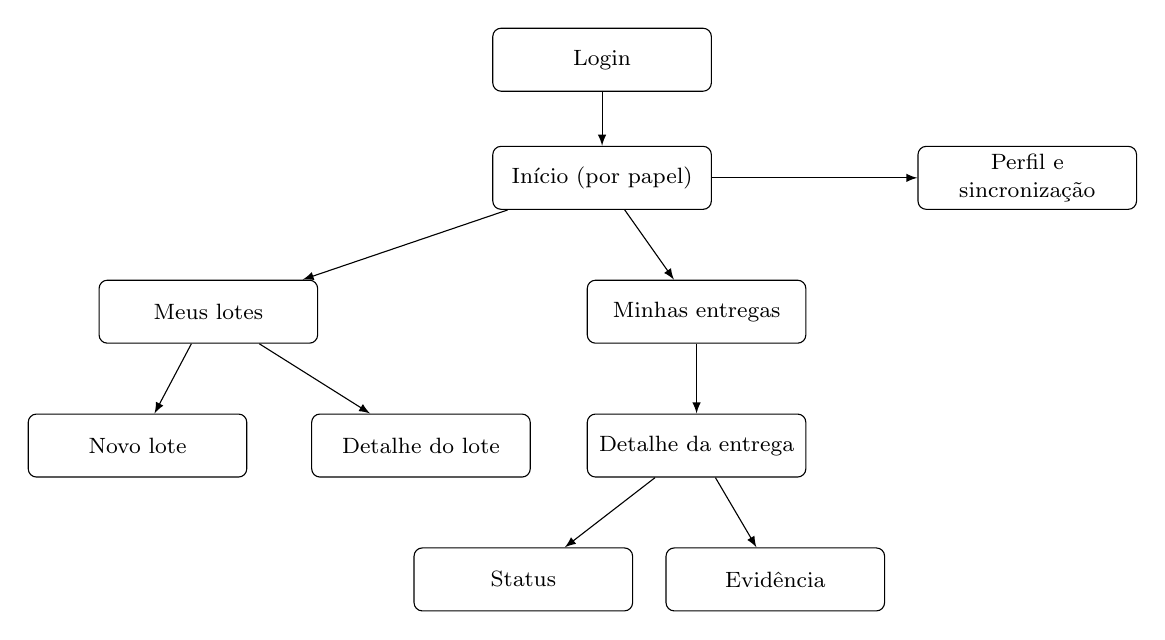
\begin{tikzpicture}[
    tela/.style={draw, rounded corners=3pt, align=center, font=\fontsize{8.5}{10}\selectfont,
      minimum height=8mm, text width=26mm, inner sep=2.5pt},
    seta/.style={-latex, thin}
  ]
    \node[tela] (login) at (0,0) {Login};
    \node[tela] (inicio) at (0,-1.5) {Início (por papel)};
    \node[tela] (lotes) at (-5.0,-3.2) {Meus lotes};
    \node[tela] (novo) at (-5.9,-4.9) {Novo lote};
    \node[tela] (dlote) at (-2.3,-4.9) {Detalhe do lote};
    \node[tela] (entregas) at (1.2,-3.2) {Minhas entregas};
    \node[tela] (dent) at (1.2,-4.9) {Detalhe da entrega};
    \node[tela] (status) at (-1.0,-6.6) {Status};
    \node[tela] (evid) at (2.2,-6.6) {Evidência};
    \node[tela] (perfil) at (5.4,-1.5) {Perfil e\\ sincronização};

    \draw[seta] (login) -- (inicio);
    \draw[seta] (inicio) -- (lotes);
    \draw[seta] (lotes) -- (novo);
    \draw[seta] (lotes) -- (dlote);
    \draw[seta] (inicio) -- (entregas);
    \draw[seta] (entregas) -- (dent);
    \draw[seta] (dent) -- (status);
    \draw[seta] (dent) -- (evid);
    \draw[seta] (inicio) -- (perfil);
  \end{tikzpicture}
  \fonte{elaborado pelo autor (2026)}
\end{figure}

\subsection{Autenticação e sessão}

O login consome o mesmo endpoint da API utilizada pela Web. Os tokens são
armazenados no \texttt{expo-secure-store}, que utiliza o armazenamento
criptográfico do sistema operacional, e não em armazenamento comum. Um
interceptador renova o token de acesso de forma transparente quando recebe 401 e
redireciona ao login apenas quando a renovação falha. No logout, os tokens e os
dados sensíveis da sessão são removidos.

\subsection{Operação offline e sincronização}

O requisito mais desafiador do aplicativo é operar sem conexão. A estratégia
combina três componentes: banco local em SQLite, fila de operações pendentes e
serviço de sincronização acionado pela mudança de conectividade.

Quando o produtor registra um lote sem sinal, o aplicativo grava o registro
localmente com estado \emph{pendente} e enfileira a operação. Quando o motorista
atualiza o status ou anexa uma evidência, o mesmo mecanismo é acionado. Ao
detectar reconexão, o serviço processa a fila em ordem, com recuo exponencial em
caso de falha temporária e limite de tentativas. A Figura~\ref{fig:sync} ilustra
o ciclo.

\begin{figure}[H]
  \centering
  \caption{Ciclo de sincronização offline}
  \label{fig:sync}
  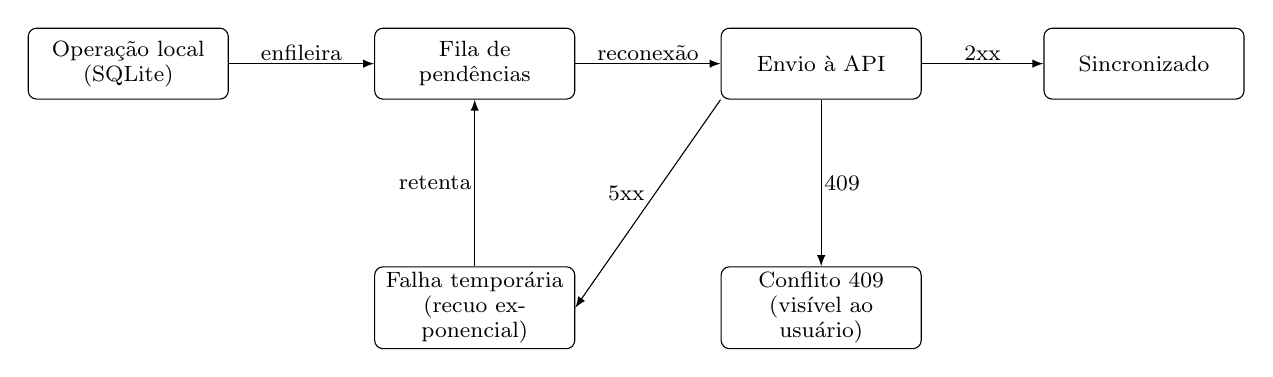
\begin{tikzpicture}[
    nodo/.style={draw, rounded corners=3pt, align=center, font=\fontsize{8}{9}\selectfont,
      minimum height=9mm, text width=24mm, inner sep=2pt},
    seta/.style={-latex, thin},
    rotulo/.style={font=\fontsize{8}{9}\selectfont, fill=white, inner sep=1pt}
  ]
    \node[nodo] (local) at (1.5,0) {Operação local\\(SQLite)};
    \node[nodo] (fila)  at (5.9,0) {Fila de\\ pendências};
    \node[nodo] (envio) at (10.3,0) {Envio à API};
    \node[nodo] (ok)    at (14.4,0) {Sincronizado};

    \node[nodo] (erro)     at (5.9,-3.1) {Falha temporária\\(recuo exponencial)};
    \node[nodo] (conflito) at (10.3,-3.1) {Conflito 409\\(visível ao usuário)};

    \draw[seta] (local) -- node[rotulo, above] {enfileira} (fila);
    \draw[seta] (fila) -- node[rotulo, above] {reconexão} (envio);
    \draw[seta] (envio) -- node[rotulo, above] {2xx} (ok);
    \draw[seta] (envio) -- node[rotulo, right] {409} (conflito);
    \draw[seta] (envio.south west) -- node[rotulo, above left] {5xx} (erro.east);
    \draw[seta] (erro) -- node[rotulo, left] {retenta} (fila);
  \end{tikzpicture}
  \fonte{elaborado pelo autor (2026)}
\end{figure}

O conflito é tratado como evento de negócio, não como erro genérico: quando o
servidor responde 409 porque o lote já foi sincronizado ou porque o status da
entrega mudou, o aplicativo marca o item como conflitante, interrompe as
tentativas automáticas e exibe a situação ao usuário. Essa decisão evita o
fenômeno de ``fila infinita'' e preserva a confiança nos dados.

\subsection{Evidência de entrega}

A evidência é composta por três elementos: fotografia, coordenadas geográficas e
observação textual. A foto pode ser capturada pela câmera ou escolhida na
galeria; antes do envio, é redimensionada e comprimida para reduzir o consumo de
dados. A localização é obtida com permissão explícita do usuário e validada
quanto à faixa de latitude e longitude.

O envio utiliza requisição multipart nativa do sistema, por meio de
\texttt{FileSystem.}\allowbreak\texttt{uploadAsync}, solução adotada após identificar que o envio
via \texttt{fetch} falhava em determinados aparelhos Android antes de atingir o
servidor. O contrato permaneceu o mesmo (\texttt{PUT
/api/v1/entregas/\{id\}/evidencia}), alterando apenas o mecanismo de transporte.
O arquivo é armazenado no servidor com nome gerado, sem confiar no nome enviado
pelo cliente.

\subsection{Testes, integração e limitações}

O aplicativo conta com 17 suítes e 79 testes automatizados, cobrindo componentes
de interface, validações, armazenamento local, fila de sincronização, conflitos e
chamadas de API. A verificação de qualidade é executada por um único comando, que
reúne análise estática, verificação de tipos e testes.

A integração real foi validada em aparelho Android 13, com a API executando
contra SQL Server e redirecionamento de porta por USB. O fluxo completo --
login do produtor, criação de lote, login do motorista, atualização de entrega e
envio de evidência com foto e GPS -- foi executado com persistência confirmada no
banco. O APK de release foi gerado com o pacote JavaScript embutido e instalado
no aparelho, funcionando sem o servidor de desenvolvimento.

Como limitações, o APK validado contempla apenas a arquitetura
\texttt{arm64-v8a}, a validação com leitor de tela TalkBack foi parcial e a
distribuição pelo EAS não foi executada por ausência de credenciais. Nenhuma
delas afeta o fluxo funcional, mas todas devem ser tratadas antes de uma
publicação em produção.
